% !TEX encoding = UTF-8
% !TEX TS-program = pdflatex
% !TEX root = ../tesi.tex

%**************************************************************
\chapter{Prodotto realizzato}
\label{cap:verifica-validazione}
In questo capitolo verrà spiegata in dettaglio come avviene l’interazione dell’utente Zendesk con l'applicazione
Zendesk e del utente Nextep con la pagina degli amministratori.

\section{Editor}
Una volta installata l'applicazione sulla piattaforma Zendesk, viene visualizzato automaticamente l'icona dell'applicazione nella sidebar della piattaforma. 
\begin{figure}[!h] 
	\centering 
	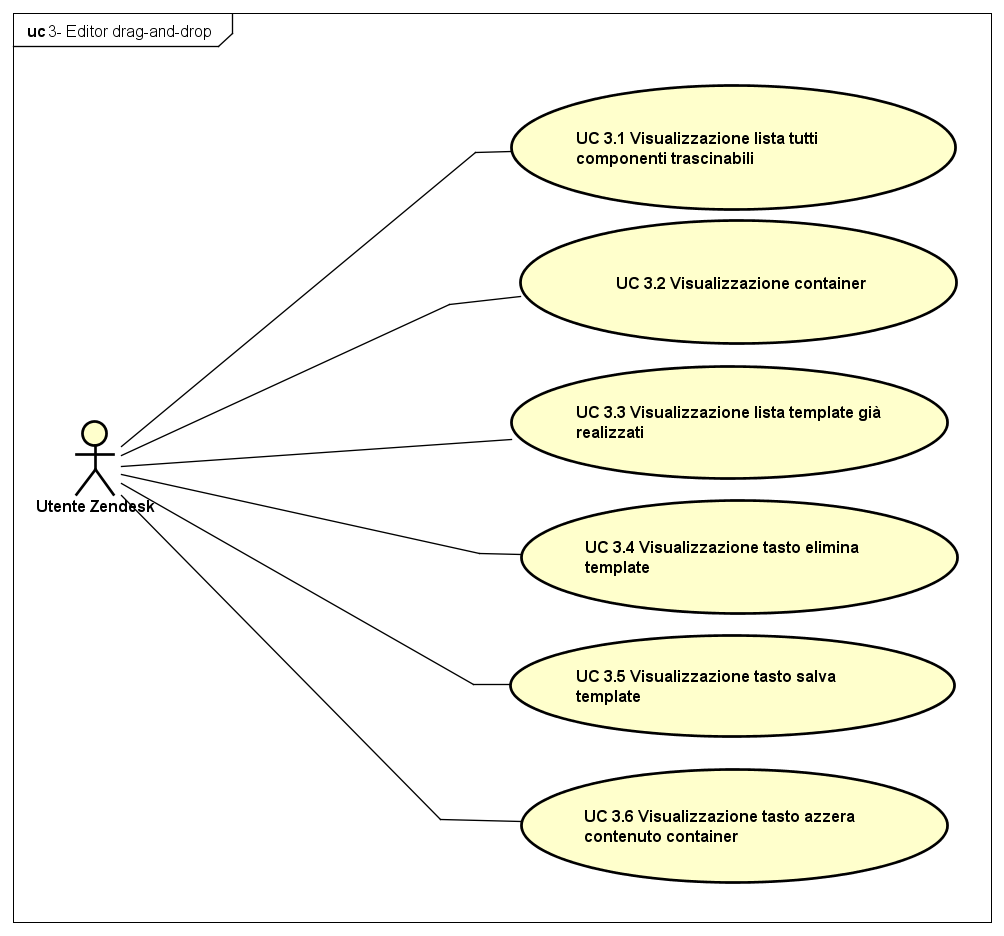
\includegraphics[width=1.2\columnwidth]{editor} 
	\caption{Editor realizzato }
\end{figure}
\begin{itemize}
	\item L'utente può trascinare qualsiasi elemento presente nei "componenti" nel container centrale;
	\item Il container visualizza a schermo il contenuto  HTML e CSS di ogni elemento trascinato in esso;
	\item Faccendo doppio click su qualsiasi elemento presente nel container centrale è possibile modificare il suo contenuto oppure eliminarlo dal container;
	\item Gli elementi nel container possono essere ordinati in qualsiasi modo semplicemente facendo drag-and-drop;
	\item E' possibile azzerrare il contenuto del container semplicemente cliccando il pulsante "Azzerra";
	\item Una volta realizzato il template deriderato l'utente può salvarlo semplicemente cliccando il pulsante "Aggiungi". Verrà chiesto all'utente di inserire il nome del template, inserito il nome valido il template verrà automaticamente salvato sul database nosql di Amazon;
	\item A destra nel "Elimina template" è possibile visualizzare tutti template realizzati e se necessario eliminarli semplicemente cliccano sull'icona "X".  
\end{itemize}
\section{Widget} 
Il widget permette al agente di Zendesk di utilizzare i template realizzati nelle risposte ai clienti. 
  \begin{figure}[!h] 
  	\centering 
  	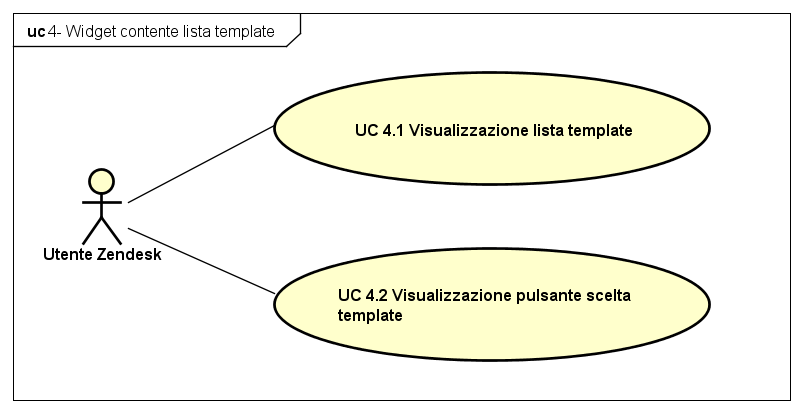
\includegraphics[width=1.2\columnwidth]{widget} 
  	\caption{Editor realizzato }
  \end{figure}
  \begin{itemize}
  	\item L'utente visualizza nel widget tutti i template realizzati;
  	\item L'utente può selezionare il template da utilizzare nella risposta;
  	\item Il template viene automaticamente aggiunto nella risposta. 
  \end{itemize}
\section{Login pagina amministratore}